\documentclass[english,man,floatsintext]{apa6}
\usepackage{lmodern}
\usepackage{amssymb,amsmath}
\usepackage{ifxetex,ifluatex}
\usepackage{fixltx2e} % provides \textsubscript
\ifnum 0\ifxetex 1\fi\ifluatex 1\fi=0 % if pdftex
  \usepackage[T1]{fontenc}
  \usepackage[utf8]{inputenc}
\else % if luatex or xelatex
  \ifxetex
    \usepackage{mathspec}
  \else
    \usepackage{fontspec}
  \fi
  \defaultfontfeatures{Ligatures=TeX,Scale=MatchLowercase}
\fi
% use upquote if available, for straight quotes in verbatim environments
\IfFileExists{upquote.sty}{\usepackage{upquote}}{}
% use microtype if available
\IfFileExists{microtype.sty}{%
\usepackage{microtype}
\UseMicrotypeSet[protrusion]{basicmath} % disable protrusion for tt fonts
}{}
\usepackage{hyperref}
\hypersetup{unicode=true,
            pdftitle={Visualisation and network analysis of physical activity and its determinants: Demonstrating opportunities using baseline associations in the Let's Move It trial},
            pdfauthor={Matti T. J. Heino, Eiko Fried, Reijo Sund, Ari Haukkala, Keegan Knittle, Katja Borodulin, Antti Uutela, Vera Araujo-Soares, Tommi Vasankari, \& Nelli Hankonen},
            pdfkeywords={exercise, physical activity, school-based intervention, behaviour change, sedentary behaviour},
            pdfborder={0 0 0},
            breaklinks=true}
\urlstyle{same}  % don't use monospace font for urls
\ifnum 0\ifxetex 1\fi\ifluatex 1\fi=0 % if pdftex
  \usepackage[shorthands=off,main=english]{babel}
\else
  \usepackage{polyglossia}
  \setmainlanguage[]{english}
\fi
\usepackage{graphicx,grffile}
\makeatletter
\def\maxwidth{\ifdim\Gin@nat@width>\linewidth\linewidth\else\Gin@nat@width\fi}
\def\maxheight{\ifdim\Gin@nat@height>\textheight\textheight\else\Gin@nat@height\fi}
\makeatother
% Scale images if necessary, so that they will not overflow the page
% margins by default, and it is still possible to overwrite the defaults
% using explicit options in \includegraphics[width, height, ...]{}
\setkeys{Gin}{width=\maxwidth,height=\maxheight,keepaspectratio}
\IfFileExists{parskip.sty}{%
\usepackage{parskip}
}{% else
\setlength{\parindent}{0pt}
\setlength{\parskip}{6pt plus 2pt minus 1pt}
}
\setlength{\emergencystretch}{3em}  % prevent overfull lines
\providecommand{\tightlist}{%
  \setlength{\itemsep}{0pt}\setlength{\parskip}{0pt}}
\setcounter{secnumdepth}{0}
% Redefines (sub)paragraphs to behave more like sections
\ifx\paragraph\undefined\else
\let\oldparagraph\paragraph
\renewcommand{\paragraph}[1]{\oldparagraph{#1}\mbox{}}
\fi
\ifx\subparagraph\undefined\else
\let\oldsubparagraph\subparagraph
\renewcommand{\subparagraph}[1]{\oldsubparagraph{#1}\mbox{}}
\fi

%%% Use protect on footnotes to avoid problems with footnotes in titles
\let\rmarkdownfootnote\footnote%
\def\footnote{\protect\rmarkdownfootnote}


  \title{Visualisation and network analysis of physical activity and its determinants: Demonstrating opportunities using baseline associations in the Let's Move It trial}
    \author{Matti T. J. Heino\textsuperscript{1*}, Eiko Fried\textsuperscript{2}, Reijo Sund\textsuperscript{3}, Ari Haukkala\textsuperscript{1}, Keegan Knittle\textsuperscript{1}, Katja Borodulin\textsuperscript{1}, Antti Uutela\textsuperscript{1}, Vera Araujo-Soares\textsuperscript{4}, Tommi Vasankari\textsuperscript{5}, \& Nelli Hankonen\textsuperscript{1}}
    \date{}
  
\shorttitle{Visualisation and network analysis in physical activity}
\affiliation{
\vspace{0.5cm}
\textsuperscript{1} Faculty of Social Sciences, University of Helsinki, PO Box 54, 00014 University of Helsinki, Finland\\\textsuperscript{2} Department of Clinical Psychology, Leiden University, Wassenaarseweg 52, 2333 AK, Leiden, The Netherlands\\\textsuperscript{3} Faculty of Health Sciences, University of Eastern Finland, PO Box 1627, 70211 Kuopio, Finland\\\textsuperscript{4} Institute of Health and Society, Medical Faculty, Newcastle University, Baddiley-Clarke Building, Richardson Road NE2 4AX, United Kindom\\\textsuperscript{5} UKK institute for Health Promotion Research, Kaupinpuistonkatu 1, 33500 Tampere, Finland}
\keywords{exercise, physical activity, school-based intervention, behaviour change, sedentary behaviour}
\usepackage{csquotes}
\usepackage{upgreek}
\captionsetup{font=singlespacing,justification=justified}

\usepackage{longtable}
\usepackage{lscape}
\usepackage{multirow}
\usepackage{tabularx}
\usepackage[flushleft]{threeparttable}
\usepackage{threeparttablex}

\newenvironment{lltable}{\begin{landscape}\begin{center}\begin{ThreePartTable}}{\end{ThreePartTable}\end{center}\end{landscape}}

\makeatletter
\newcommand\LastLTentrywidth{1em}
\newlength\longtablewidth
\setlength{\longtablewidth}{1in}
\newcommand{\getlongtablewidth}{\begingroup \ifcsname LT@\roman{LT@tables}\endcsname \global\longtablewidth=0pt \renewcommand{\LT@entry}[2]{\global\advance\longtablewidth by ##2\relax\gdef\LastLTentrywidth{##2}}\@nameuse{LT@\roman{LT@tables}} \fi \endgroup}


\usepackage{lineno}

\linenumbers

\authornote{Trial Registration Number: ISRCTN10979479. Registered retrospectively: 31.12.2015

Correspondence concerning this article should be addressed to Matti T. J. Heino, . E-mail: \href{mailto:matti.tj.heino@gmail.com}{\nolinkurl{matti.tj.heino@gmail.com}}}

\abstract{
Background: Let's Move It is a complex whole-school system intervention aiming to reduce sedentary behaviours (SB) and increase physical activity (PA) among adolescents in vocational schools, by targeting their environmental and psychosocial determinants. This paper describes participants' baseline characteristics in a cluster-randomised trial testing the Let's Move It intervention, and explores possibilities for visual data presentation, making use of recent developments in software and network analyses. We provide an example of a comprehensive research report with all analysis code and results in a readily accessible format, for researchers to apply these tools to other data. Methods: At baseline, 1166 adolescents in 57 classes at 6 school units, distributed across four educational tracks, participated the study. We measured health status, activity and inactivity, as well as psychological and social constructs possibly mediating effects of the intervention on outcomes, with 7-day accelerometry, bioimpedance measures, and questionnaires. Data were visualized using various techniques, e.g., combining ridge plots and diamond plots. Network analysis was used to explore relations between psychological/social variables and outcomes. Results: Mean age of participants was 18.8 (Md = 17.0) years. On average, participants engaged in moderate-to-vigorous daily PA for 1h 29min (CI95: 1h 19min - 1h 40min), SB for 9h 34min (CI95: 8h 56min - 10h 12min), and interrupted sitting 28 times (CI95: 24.7 - 31.4) per day on average. Randomization appeared to result in balanced distributions for baseline characteristics between intervention and control groups , but differences emerged across the four educational tracks. Self-reported behaviour change technique (BCT) use was low for many but not all techniques. In network analysis with a network consisting of BCTs, motivation and PA , behavioural experiments, planning and autonomous motivation were directly related to PA, and several BCTs were connected via autonomous motivation. Conclusion: Grasping the dynamics of complex multicausal systems is a challenging task, which can be aided by data-visualization and data exploration (e.g.~via network analysis). We discuss benefits of presenting complex data visually to encourage researchers to publish extensive analyses and descriptions as website supplements. That would increase speed and quality of scientific communication, and may address recent concerns of reduced confidence towards research findings.


}

\begin{document}
\maketitle

\newpage

\hypertarget{background}{%
\section{Background}\label{background}}

Declining physical activity (PA) and increasing sedentary behaviour (SB) are costly and growing concerns for public health, studies indicating a higher risk for individuals with low socioeconomic status (SES) {[}1{]}. Patterns of low PA among adults begin earlier in the life course, with evidence that declines in PA and increases in SB begin during childhood and adolescence {[}3,4{]}. This highlights the need for further research into interventions to improve PA and SB among adolescents.

As adolescents spend a significant amount of their time in schools, the school setting provides valuable opportunities for PA and SB interventions {[}5{]}. The Let's Move It intervention aimed to reduce SB and increase PA among adolescents in vocational schools, and was developed using stakeholder input and co-creation with target group representatives, as well as theories and empirical evidence from behavioural science {[}6,7{]}. Contrary to typical school-based interventions with relatively homogeneous participants, this trial was carried out in vocational schools with varied and distinct educational tracks (i.e.~practical nurse, business information and communication technology, business administration, and hotel, restaurant and catering). Understanding the implications of these distinct tracks on the way participants engage in both PA and SB will support a better understanding of the individual and contextual determinants of behaviour and more informed interpretations of the results obtained in the trial.

The hypothesised programme theories {[}8,9{]} for changing PA and SB differed from one another. In order to increase PA, one needs to make a conscious effort and implement self-regulatory skills (e.g.~action planning and overcoming barriers to PA) to make optimal use of opportunities. The Let's Move it intervention places a particular emphasis on helping adolescents understand and use techniques to manage their motivation and behaviour (see also {[}10{]}). To date, there is little knowledge about how the use of these techniques links to each other, and it would be important to examine these links empirically. The theoretical model for changing SB, on the other hand, is more driven by environmental opportunities, such as having the option of standing up during class.

In order to increase moderate-to-vigorous-intensity PA, the Let's Move It intervention targeted several mediating behavioral determinants, including behavioural beliefs (outcome expectations, descriptive norms, intention, self-efficacy/perceived behavioural control), autonomous and controlled motivation, environmental opportunities, action and coping planning, and behaviour change technique (BCT) use. Key hypotheses regarding students' PA change have been registered in OSF (\url{https://osf.io/tb8fu/}). To reduce total SB and introduce breaks in SB, the programme aimed to change the school environment by training teachers in the use of active teaching techniques and altering physical choice architecture in classrooms {[}11{]}. The intervention included also poster campaigns in schools, and a website, as well as materials to target community actors and parents {[}11{]}. More information of the content of the intervention and the development of it is reported elsewhere ({[}10{]}, Hankonen et al.~unpublished manuscript).

It has long been a standard recommendation for quantitative analyses to investigate data visually as a core precursor of conducting statistical analyses {[}12,13{]}. However, in social and life sciences, such visualisations have rarely been shared in publications. Information about data are usually limited to means and standard deviations, which presents at best limited information about the variables of interest. Medians, modes, skewness and kurtosis provide helpful additional information, but human cognition places limits on evaluating these statistics simultaneously, especially when comparing groups of observations. For example, two distributions can have different means but the same mode, different modes but the same mean, same mean and standard deviation but a meaningful skew, et cetera. Summary statistics conventionally calculated from the data leave important distributional properties uncovered, as illustrated in recent discussions on the inadequacy of bar plots {[}14--16{]}.

Data visualisation is crucial to supplement possibly large numerical tables of descriptive statistics {[}17{]}. With visualisations, researchers can communicate large amounts of information -- including the associated uncertainty -- in an accessible format, without requiring extensive mathematical expertise from the reader. This is important for researchers who intend to build on previous results {[}18{]}. Such practices may be a way to reduce problems that have led to the recent loss of confidence in the reproducibility and replicability of research findings {[}19--28{]}. The ideal would be to share fully open data, but this is not always possible due to privacy concerns {[}29{]} and, at the time of writing, a lamentably rare practice {[}30{]}. In addition, open data does not necessarily accommodate stakeholders with low technical expertise in data analysis and visualisation, such as clinicians, patients and policy makers; see {[}31{]}, p.~2.

Three recent developments give impetus to a new approach. First, many journals now allow publication of supplementary online materials, which circumvents both word and figure restrictions of traditional manuscripts. Second, statistical software such as R {[}32{]} has recently become increasingly mainstream among applied researchers, with many free tutorials available online, opening the door also for a variety of data visualisation techniques. Third, novel statistical methods in social and health psychology, such as psychological network analysis, may help to understand relationships between variables, by making better use of visual representations of associations.

The aims of this paper are to describe central characteristics of the Let's Move It trial baseline cohort, focusing on co-primary outcomes and other activity measures (as measured by accelerometry) of the trial both arms, genders and educational tracks in both trial arms. A further aim is to describe psychological and social correlates, as well as hypothesised determinants of the intervention effect on moderate-to-vigorous physical activity, with detailed visualisations of the dataset provided in an extensive supplement. As a subaim, we also investigate network of relationships between moderate-to-vigorous intensity physical activity (MVPA), quality of motivation and BCT use at baseline. We provide all code as open source scripts so that other researchers can use those scripts as templates to deliver visualized information in a format that requires no special skills or tools to view.

\hypertarget{methods}{%
\section{Methods}\label{methods}}

This study analyzes baseline data from a cluster-randomised controlled trial testing Let's Move It, a complex whole-school system multi-level intervention conducted in Finnish vocational schools. Details of Let's Move It trial have been described in the study protocol {[}33{]}. At baseline, consenting participants in both intervention and control groups answered an electronic survey, underwent bioimpedance measurements and were instructed to wear an accelerometer for seven consecutive days.

Six school units were included in the study. There were four educational tracks in the schools from which students were recruited: 1. Practical Nurse (Nur), 2. Hotel, Restaurant and Catering (HRC), 3. Business and Administration (BA), and 4. Information and Communications Technology (IT). Schools were paired so that there would be matching numbers of students from each educational track for both members of the pair. Blinded randomization by a statistician was then conducted so that a random member of each pair was selected as intervention school, the other as control school (details reported in {[}33{]}). Student participants were blind to allocation at baseline.

All conducted analyses and visualisations with accompanying code, can be found in the supplementary website at \url{https://git.io/fNHuf} (permalink at {[}REF, to be added right before submission{]}). Source code to reproduce this manuscript and all its figures can be found at \url{https://git.io/fptcC}.

\hypertarget{measures}{%
\subsection{Measures}\label{measures}}

The measures are presented briefly, as they have been previously described in {[}33{]}, and all individual items of the scales are available in the supplementary file {[}todo: add direct link{]}.

\hypertarget{primary-outcome-variables-of-the-trial}{%
\subsubsection{Primary outcome variables of the trial}\label{primary-outcome-variables-of-the-trial}}

In the LMI trial, the primary outcome for PA was moderate to vigorous PA (MVPA), measured by accelerometry and self-reports. Primary outcomes for sedentary behaviour (SB) were measured by accelerometry. They included time spent sitting or lying down, and the number of times sitting was interrupted during the day.

\emph{Self-reported MVPA.} Self-reported MVPA was measured with two questions in accordance with the NordPAQ measurement {[}34{]}. The first question asked participants about the number of days during the last week in which they did more than 30 minutes of MVPA, the other probed the overall amount of MVPA (in hours) during the past seven days.

\emph{Accelerometer-measured MVPA and SB.} No more than seven days after responding to the questionnaire, students were given an accelerometer to be worn on seven consecutive days. The hip-worn accelerometer (Hookie AM 20, Traxmeet Ltd, Espoo, Finland) using a digital triaxial acceleration sensor (ADXL345; Analog Devices, Norwood MA) was attached to a flexible belt and participants were instructed to wear the belt around their right hip for seven consecutive days during waking hours, except during shower and other water activities. The acceleration signal was collected at 100 Hz sampling frequency, \(\pm\) 16 g acceleration range and 0.004 g resolution. PA-parameters were based on mean amplitude deviation (MAD) of the resultant acceleration analysed in 6s epochs {[}35{]}. The MAD values were then converted to metabolic equivalent (MET) values {[}36{]}. The epoch-wise MET values were further smoothed by calculating 1min exponential moving average. Using the smoothed MET values total PA was classified in terms of energy consumption covering MET values higher than 1.5 and moderate-to-vigorous PA (MVPA) covering MET values equal to or higher than 3 {[}35,36{]}. According to the definition of SB {[}37{]}, time spent in sitting and reclining positions were combined to indicate SB, whereas standing was analysed separately as another form of stationary behaviour. Body postures were recognized from the raw acceleration data by employing both direction and intensity information from all three measurement axes. The recognition was based on the low intensity of movement (\textless{}1.5 MET) and the accelerometer orientation in relation to identified upright position (angle for posture estimation, APE) calculated at the end of each 6 s epoch {[}38{]}.

\hypertarget{theoretical-predictors-of-pa}{%
\subsubsection{Theoretical predictors of PA}\label{theoretical-predictors-of-pa}}

The mediators postulated by the program theory included behavioural beliefs (outcome expectations, descriptive norms, intention, self-efficacy/perceived behavioural control), autonomous and controlled motivation, opportunities, action- and coping planning, and behaviour change technique (BCT) use. Participants were allowed to skip questions, and scales were computed as means of all items where responses were available. In other words, answering a single item sufficed. All items, response options, and descriptive statistics of scales are available in the supplementary website (\url{https://git.io/fAj0e}).

\hypertarget{statistical-analysis}{%
\subsubsection{Statistical analysis}\label{statistical-analysis}}

We used RStudio {[}39{]} 1.1.456 running R {[}40{]} 3.5.1 for all our analyses and figures.

In our case (no confirmatory hypotheses), confidence intervals are more appropriate to report than p-values, as they provide readily interpretable values on the same scale as the original variable, accommodating inferences of practical relevance {[}23,41--43{]}. Hence, we omit explicit statistical testing from the tables.

Activity data was explored by utilising 100\% stacked bar charts, which are useful when comparing proportions which add to 100\%. MVPA data was, in addition, examined with augmented raincloud ridge plots to unveil distributional properties. Psychological and social determinants were examined with diamond plots, and heuristic effect sizes between means of intervention arms and genders transformed from Cohen's d to Pearson's r. Distributions of BCT use were examined with histograms.

Psychological network analysis was used to estimate and visualise relations among BCT use, motivation and MVPA. Such networks contain nodes (variables) and edges (statistical relationships between variables). Unlike in social network analysis, the connections are not directly observed, but are estimated. We used network models that estimate conditional dependence relations among a set of variables, which can be interpreted similarly to partial correlations. An edge between two variables implies that they are related after controlling for all other variables; the absence of an edge implies that the two variables are (conditionally) independent.

The Mixed Graphical Model uses regularization, a procedure that has been shown to help recover the true network structure in data in case the data were simulated under a network model {[}44{]}. Regularization has the goal to avoid estimating spurious relationships among items (i.e.~false positive relations), and results in a parsimonious network structure. The regularization technique used here is the Least Absolute Shrinkage and Selection Operator (LASSO; {[}45{]}), which shrinks all edges and sets very small edges to exact zero. A paper that explains lasso regularization in network models in detail can be found elsewhere {[}46{]}.

Network models applied to between-subjects data at one time-point can be useful for describing health psychological data, as well as facilitating group-level hypothesis generation regarding which parts of the system are central for a problem at hand {[}47{]}. Identifying these determinants of importance can thus supplement traditional structural equation modeling (SEM) approaches. Network analysis has recently been taken up in many fields such as social psychology {[}48,49{]}, personality {[}50{]}, intelligence {[}51{]}, psychopathology {[}52{]}, and empathy research {[}53{]}, and is beginning to be applied for health behaviours on a broader scale. Several helpful tutorial papers aimed at empirical researchers are available {[}46,54--57{]}, and also exist for health psychology context in particular {[}58{]}.

To ease interpretation of the network analysis, we dichotomised the heavily skewed controlled motivation dimension in such a way that 1 represents answers 3 (\enquote{partly true for me}) or higher, and 0 the rest. In addition, BCT use variables were dichotomised by giving 0 if a person reports completely disagreeing with their statements, or never having used the technique, and 1 otherwise. A correlation matrix of the variables can be found in the supplement (\url{https://git.io/fhAgk}).

\hypertarget{findings}{%
\section{Findings}\label{findings}}

In this section, we first present data in traditional numeric tables, and follow up by augmenting them with graphical illustrations. Table \ref{tab:demographics-table} shows the main demographic variables of the cohort by educational track. Most (83.1\%) participants were born in Finland. While on average the sample consist of both boys and girls (43.5\% vs.~56.5\%), educational tracks were heavily divided by gender: Practical Nurse track had the highest amount of girls (82.3\%) and IT track lowest (16.0\%). Age ranged from 16 to 49, with the average age being 18.50. Altogether there were 190 (16\%) students who reported being at least 20 years old.

\begin{table}[tbp]
\begin{center}
\begin{threeparttable}
\caption{\label{tab:demographics-table}Baseline demographics of educational tracks.}
\begin{tabular}{llllll}
\toprule
Variable & \multicolumn{1}{c}{Nur} & \multicolumn{1}{c}{HRC} & \multicolumn{1}{c}{BA} & \multicolumn{1}{c}{IT} & \multicolumn{1}{c}{Full sample}\\
\midrule
n & 402 & 213 & 282 & 163 & 1166\\
Mean study year (sd, median) & 1.7 (0.9, 1.0) & 1.9 (0.7, 2.0) & 1.7 (0.9, 1.0) & 1.7 (0.9, 1.0) & 1.7 (0.9, 1.0)\\
Mean age (range, median) & 18.8 (16.0-49.0, 17.0) & 18.5 (17.0-27.0, 18.0) & 18.0 (16.0-35.0, 17.0) & 18.5 (17.0-43.0, 17.0) & 18.5 (16.0-49.0, 18.0)\\
Born in Finland (\%) & 80.0 & 88.2 & 87.1 & 87.9 & 83.1\\
\% girl & 82.3 & 60.6 & 39.0 & 16.0 & 56.5\\
\% allocated to intervention & 68.9 & 31.5 & 53.5 & 46.6 & 54.7\\
\bottomrule
\addlinespace
\end{tabular}
\begin{tablenotes}[para]
\normalsize{\textit{Note.} Omitted are 24 participants, who reported "other" as their track, as well as 81 participants from whom the data is not available. Nur = Practical nurse, HRC = Hotel, restaurant and catering studies, BA = Business and administration, IT = Business information technology.}
\end{tablenotes}
\end{threeparttable}
\end{center}
\end{table}

Table \ref{tab:primary-outcome-vars-table-total} shows summary statistics for primary outcome variables with their intra-class correlations (ICCs) for class and school (see supplementary website for ICCs for all variables). The ICC can be interpreted as the proportion of the variable's variance, which can be accounted for by group membership.

At baseline, 63.6\% students provided at least 4 days with a minimum of 10 hours per day of valid accelerometer data. On average, the participants reported engaging in at least 30 minutes of MVPA on 2.80 days a week. Accelerometer data indicated, that girls were slightly more active than boys (mean 65 vs.~67 minutes). Given that boys are generally more active than girls {[}3{]}, this result will be elaborated on below.

\begin{table}[tbp]
\begin{center}
\begin{threeparttable}
\caption{\label{tab:primary-outcome-vars-table-total}Primary outcome variables with their class and school ICCs. Accelerometer results, including wear time, are only included from those participants who met the cutoff of at least 10 hours of measurement time for at least four days.}
\begin{tabular}{llllll}
\toprule
Variable & \multicolumn{1}{c}{Mean} & \multicolumn{1}{c}{CI95} & \multicolumn{1}{c}{ICC class} & \multicolumn{1}{c}{ICC school} & \multicolumn{1}{c}{n}\\
\midrule
Daily moderate-to-vigorous PA time (accelerometer)* & 1h 5min & 0h 57min - 1h 13min & .089 & .062 & 731\\
Daily light PA time (accelerometer) & 2h 51min & 2h 32min - 3h 9min & .111 & .110 & 731\\
Daily standing time (accelerometer) & 1h 24min & 1h 15min - 1h 34min & .122 & .041 & 731\\
Daily time spent sitting or lying down (accelerometer)* & 8h 44min & 8h 4min - 9h 24min & .115 & .138 & 731\\
Daily number of times sitting was interrupted (accelerometer)* & \ \ 25.8 & \ \ 23.5\ \ -\ \ \ \ 28.0 & .047 & .080 & 731\\
Number of days with >30 MVPA min previous week (self-report)* & \ \  2.8 & \ \  2.6\ \ -\ \ \ \  3.0 & .047 & < .001 & 1082\\
\bottomrule
\addlinespace
\end{tabular}
\begin{tablenotes}[para]
\normalsize{\textit{Note.} *Primary outcome variables. Accelerometry data missing from 435, and survey data from 84 participants.}
\end{tablenotes}
\end{threeparttable}
\end{center}
\end{table}

To give the reader a richer perspective than from what can be gauged from considering these summary statistics only, we present the results graphically in figure \ref{fig:average-day-activity-plot}. We can see that the patterns of average baseline activity, as measured by the accelerometer, are similar within gender and intervention allocation groups. However, the charts reveal that the IT track is more sedentary compared to other tracks and that girls are actually \emph{less} active in each educational track.

\begin{figure}
\centering
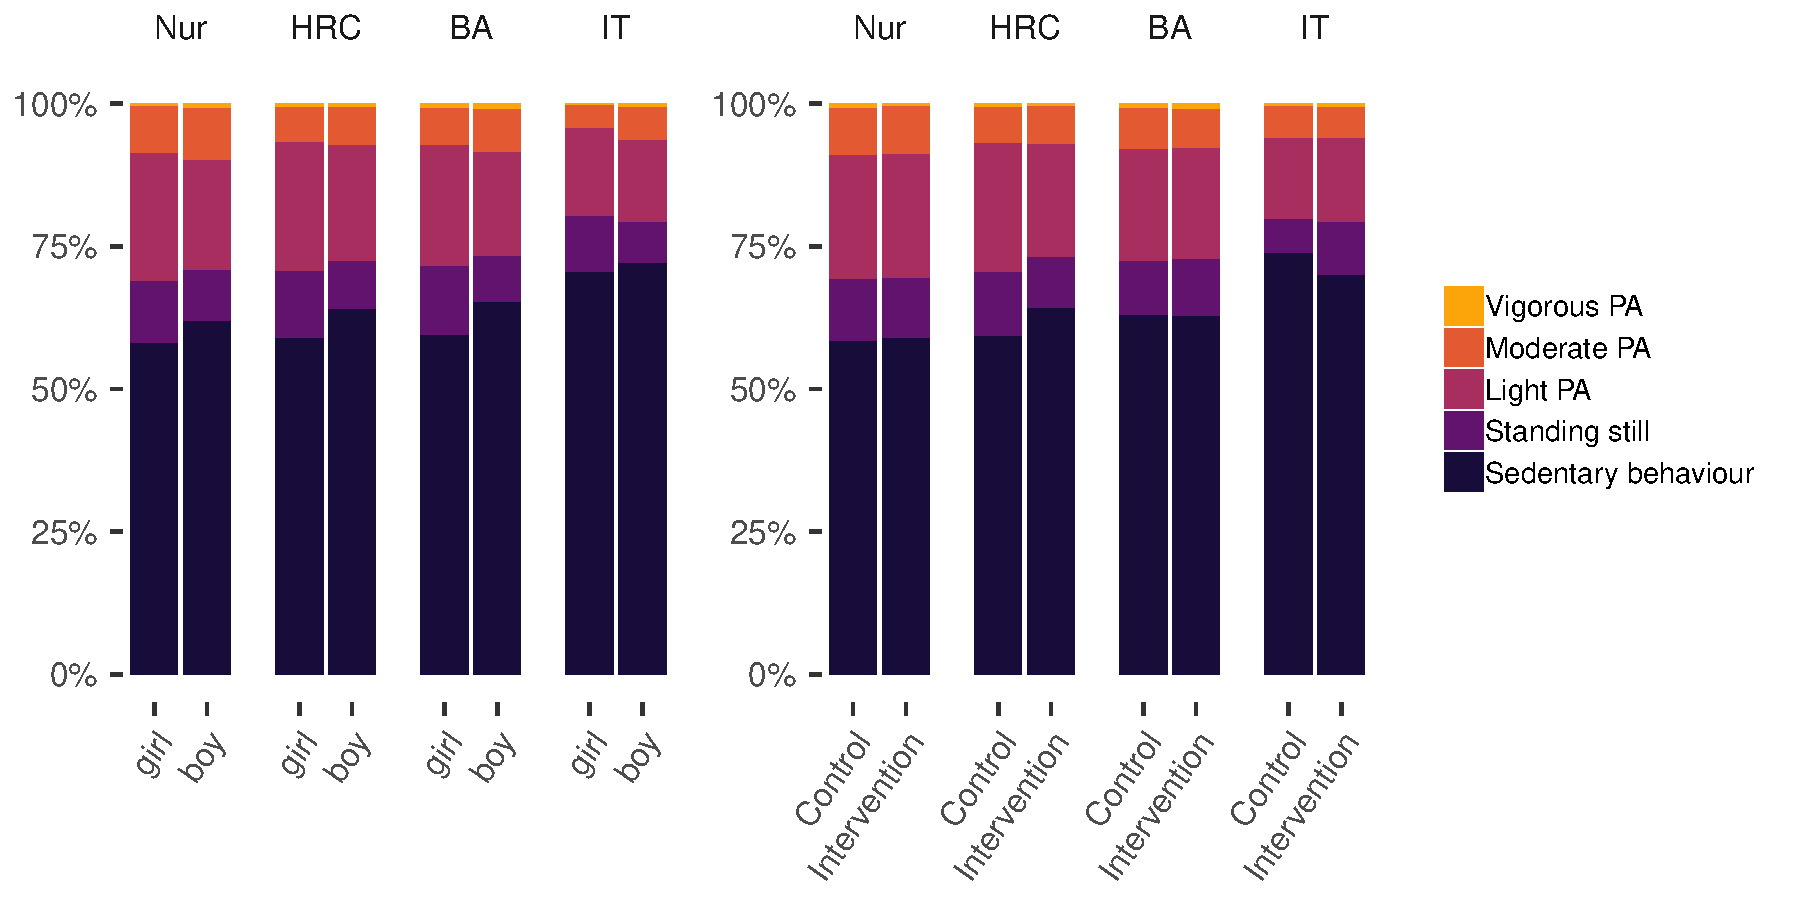
\includegraphics{_baseline-manuscript_files/figure-latex/average-day-activity-plot-1.pdf}
\caption{\label{fig:average-day-activity-plot}Stacked bar plot drawn with R package \texttt{ggplot} (code available at \url{https://git.io/fptlp}), showing proportions of accelerometer-measured activity in relation to measurement time, averaged over genders, arms and educational tracks. Nur = Practical nurse, HRC = Hotel, restaurant and catering, BA = Business and administration, IT = Information and communications technology.}
\end{figure}

The plot shows the average activity types relative to measurement time, but hides variability around the averages. The graph does not depict, for example, that while the average portion of time spent in sedentary behaviour for the IT track was 72.0\%, almost half (42.0\%) of that track's participants were sedentary more than 75\% of the time.

Zooming in on accelerometer-measured MVPA, table \ref{tab:mvpa-table} gives us statistics -- some of which more commonly reported, others less so -- on the variable.

\begin{table}[tbp]
\begin{center}
\begin{threeparttable}
\caption{\label{tab:mvpa-table}Statistics describing MVPA in different educational tracks. Values not corrected for effects of clustering.}
\begin{tabular}{llllll}
\toprule
Gender & \multicolumn{1}{c}{Arm} & \multicolumn{1}{c}{Nur} & \multicolumn{1}{c}{HRC} & \multicolumn{1}{c}{BA} & \multicolumn{1}{c}{IT}\\
\midrule
girl & control & M=73.0; SD=29.5; skewness=0.9; kurtosis= 0.6; n=104 & M=57.5; SD=22.3; skewness=0.8; kurtosis= 1.0; n=90 & M=61.2; SD=23.8; skewness=0.8; kurtosis= 1.0; n=53 & M=34.2; SD= 8.9; skewness=0.4; kurtosis=-0.8; n=14\\
girl & intervention & M=71.8; SD=28.4; skewness=1.0; kurtosis= 1.6; n=227 & M=52.0; SD=23.6; skewness=0.8; kurtosis=-0.2; n=39 & M=58.7; SD=22.8; skewness=1.2; kurtosis= 0.7; n=57 & M=36.1; SD=22.1; skewness=0.2; kurtosis=-0.8; n=12\\
boy & control & M=72.7; SD=28.9; skewness=0.3; kurtosis=-1.1; n=21 & M=56.1; SD=27.4; skewness=1.5; kurtosis= 2.0; n=56 & M=70.4; SD=27.3; skewness=0.7; kurtosis= 0.6; n=78 & M=55.2; SD=25.2; skewness=1.2; kurtosis= 2.8; n=73\\
boy & intervention & M=89.6; SD=39.1; skewness=0.7; kurtosis= 0.2; n=50 & M=71.2; SD=43.9; skewness=0.9; kurtosis= 0.5; n=28 & M=72.1; SD=31.1; skewness=0.5; kurtosis=-0.8; n=94 & M=54.5; SD=25.3; skewness=1.2; kurtosis= 1.4; n=64\\
\bottomrule
\end{tabular}
\end{threeparttable}
\end{center}
\end{table}

Figure \ref{fig:MVPA-accelerometer-plot} displays an augmented density plot, representing and elaborating on information from table \ref{tab:mvpa-table}. The density curves can be read like a histogram, but the shape is not dependent on the bar width. They also help illustrate differences across groups, revealing potential differences in variability and distribution shape.

\begin{figure}
\centering
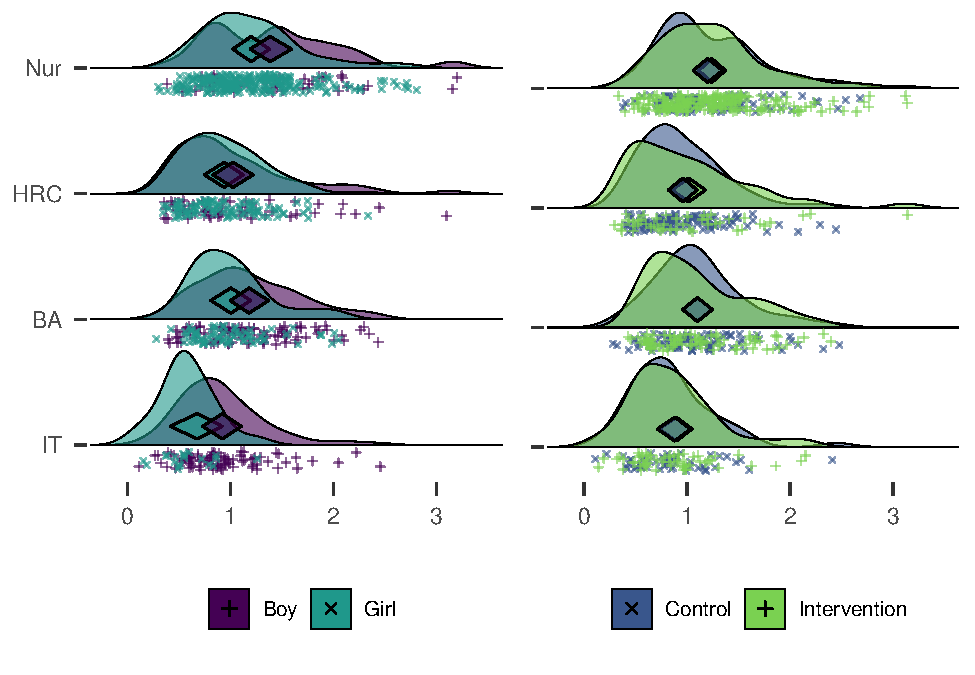
\includegraphics{_baseline-manuscript_files/figure-latex/MVPA-accelerometer-plot-1.pdf}
\caption{\label{fig:MVPA-accelerometer-plot}Raincloud ridge plot combined with a diamond plot, drawn with R packages \texttt{ggridges} and \texttt{userfriendlyscience} (code available at \url{https://git.io/fpt4c}), showing hours of MVPA for different educational tracks. Midpoints of diamonds indicate means, endpoints 95\% credible intervals (see {[}{\textbf{???}}{]} for interpretation). Individual observations are presented under the density curves, with random scatter on the y-axis to ease inspection. Nur = Practical nurse, HRC = Hotel, restaurant and catering, BA = Business and administration, IT = Information and communications technology.}
\end{figure}

As can be seen from the x-axis placement of diamonds in figure \ref{fig:MVPA-accelerometer-plot}, participants who study practical nurssing are the most active, followed by HRC students and BA students, with the IT track being the least active. There is considerable variation within tracks though. This explains the gender difference in MVPA: the practical nurse track is the largest, and its students, mostly girls, are the most active. The IT students, mostly boys, are the least active.

In sum, boys did more MVPA in every educational track (mean differences in minutes: 12.80 for Practical nurse, 5.40 for Hotel, restaurant and catering, 11.30 for Business and administration, and 19.80 for IT). In spite of this, girls appear more active in the aggregate. This is also known as the Simpson's paradox, and is best investigated by visualising data (see {[}59{]} for an introduction). Examining the left side of figure \ref{fig:MVPA-accelerometer-plot} reveals the difference between boys and girls in MVPA, the difference between Practical nurse and IT tracks, the differences in gender decomposition, and differences in the amount of participants in each track which, put together, contributes to a comprehensive understanding of the data.

Similar plots for all primary outcome variables can be found in the supplement. In brief, regardless of track, boys reported more days with at least 30 minutes of MVPA, while reporting more e.g.~gym training, which was more strongly connected to the self-reported MVPA than the accelerometer-measured one. Accelerometer measurement also indicated, that boys engaged in more sedentary time and interrupted sitting less often than girls. These results are also described in the supplement.

\hypertarget{theoretical-determinants}{%
\subsection{Theoretical determinants}\label{theoretical-determinants}}

In table \ref{tab:mediator-table} below, we present the means for the primary outcome variables by gender and trial arm.

\begin{table}[tbp]
\begin{center}
\begin{threeparttable}
\caption{\label{tab:mediator-table}Main theoretical determinants of PA and SB. Mean (CI95).}
\begin{tabular}{llllll}
\toprule
Variable  & \multicolumn{1}{c}{Girls (n = 603-611)} & \multicolumn{1}{c}{Boys (n = 459-467)} & \multicolumn{1}{c}{Intervention (n = 570-579)} & \multicolumn{1}{c}{Control (n = 492-499)} & \multicolumn{1}{c}{Total (n = 1062-1078)}\\
\midrule
PA intention & 5.3 (5.1 - 5.5) & 5.5 (5.2 - 5.7) & 5.4 (5.1 - 5.7) & 5.4 (5.1 - 5.7) & 5.4 (5.2 - 5.6)\\
PA perceived behavioural control & 5.2 (5.1 - 5.3) & 5.5 (5.4 - 5.6) & 5.3 (5.1 - 5.5) & 5.3 (5.1 - 5.5) & 5.3 (5.2 - 5.5)\\
PA self-efficacy & 5.1 (5.0 - 5.3) & 5.3 (5.2 - 5.5) & 5.2 (5.0 - 5.3) & 5.3 (5.1 - 5.4) & 5.2 (5.1 - 5.4)\\
PA opportunities & 5.1 (5.0 - 5.1) & 5.2 (5.1 - 5.3) & 5.1 (5.0 - 5.2) & 5.2 (5.1 - 5.3) & 5.1 (5.1 - 5.2)\\
PA descriptive norm & 4.3 (4.1 - 4.5) & 4.6 (4.4 - 4.7) & 4.3 (4.1 - 4.5) & 4.5 (4.3 - 4.7) & 4.4 (4.2 - 4.6)\\
PA injunctive norm & 4.6 (4.4 - 4.8) & 4.8 (4.5 - 5.0) & 4.5 (4.3 - 4.7) & 4.8 (4.6 - 5.0) & 4.7 (4.5 - 4.8)\\
PA outcome expectations & 5.4 (5.2 - 5.5) & 5.1 (5.0 - 5.3) & 5.2 (5.0 - 5.5) & 5.3 (5.1 - 5.5) & 5.3 (5.1 - 5.4)\\
PA action planning & 2.7 (2.6 - 2.8) & 2.8 (2.7 - 2.9) & 2.7 (2.6 - 2.8) & 2.8 (2.7 - 2.9) & 2.8 (2.7 - 2.8)\\
PA coping planning & 2.4 (2.4 - 2.5) & 2.6 (2.5 - 2.7) & 2.5 (2.4 - 2.6) & 2.5 (2.4 - 2.6) & 2.5 (2.4 - 2.6)\\
PA autonomous regulation & 3.3 (3.2 - 3.5) & 3.6 (3.4 - 3.7) & 3.4 (3.2 - 3.5) & 3.5 (3.3 - 3.6) & 3.4 (3.3 - 3.5)\\
PA controlled regulation & 1.9 (1.8 - 2.0) & 1.8 (1.7 - 1.8) & 1.8 (1.7 - 1.9) & 1.9 (1.8 - 1.9) & 1.8 (1.8 - 1.9)\\
PA amotivation & 1.5 (1.4 - 1.5) & 1.6 (1.5 - 1.7) & 1.5 (1.4 - 1.6) & 1.5 (1.4 - 1.6) & 1.5 (1.5 - 1.6)\\
PA agreement-BCTs & 3.1 (2.9 - 3.2) & 3.2 (3.0 - 3.3) & 3.0 (2.9 - 3.2) & 3.2 (3.0 - 3.4) & 3.1 (3.0 - 3.2)\\
PA frequency-BCTs & 2.5 (2.4 - 2.6) & 2.6 (2.4 - 2.7) & 2.5 (2.4 - 2.6) & 2.6 (2.4 - 2.7) & 2.5 (2.4 - 2.6)\\
SB intention & 3.8 (3.5 - 4.1) & 3.6 (3.3 - 3.9) & 3.7 (3.2 - 4.2) & 3.7 (3.3 - 4.2) & 3.7 (3.4 - 4.1)\\
SB descriptive norm & 3.2 (3.0 - 3.4) & 3.4 (3.1 - 3.6) & 3.2 (3.0 - 3.4) & 3.3 (3.1 - 3.5) & 3.2 (3.1 - 3.4)\\
SB injunctive norm & 4.0 (3.8 - 4.1) & 4.1 (3.9 - 4.3) & 3.9 (3.8 - 4.1) & 4.1 (4.0 - 4.2) & 4.0 (3.9 - 4.1)\\
SB outcome expectations & 4.9 (4.8 - 5.0) & 4.5 (4.4 - 4.7) & 4.8 (4.5 - 5.0) & 4.8 (4.6 - 5.0) & 4.8 (4.6 - 4.9)\\
\bottomrule
\end{tabular}
\end{threeparttable}
\end{center}
\end{table}

In 14 of the 19 variables presented here, the mean of the control group is more favourable than that of the intervention group (average unadjusted advantage 1.75\%). In figure \ref{fig:determinant-diamondplot-manuscript}, the results are visualised in a concise manner.

\begin{figure}
\centering
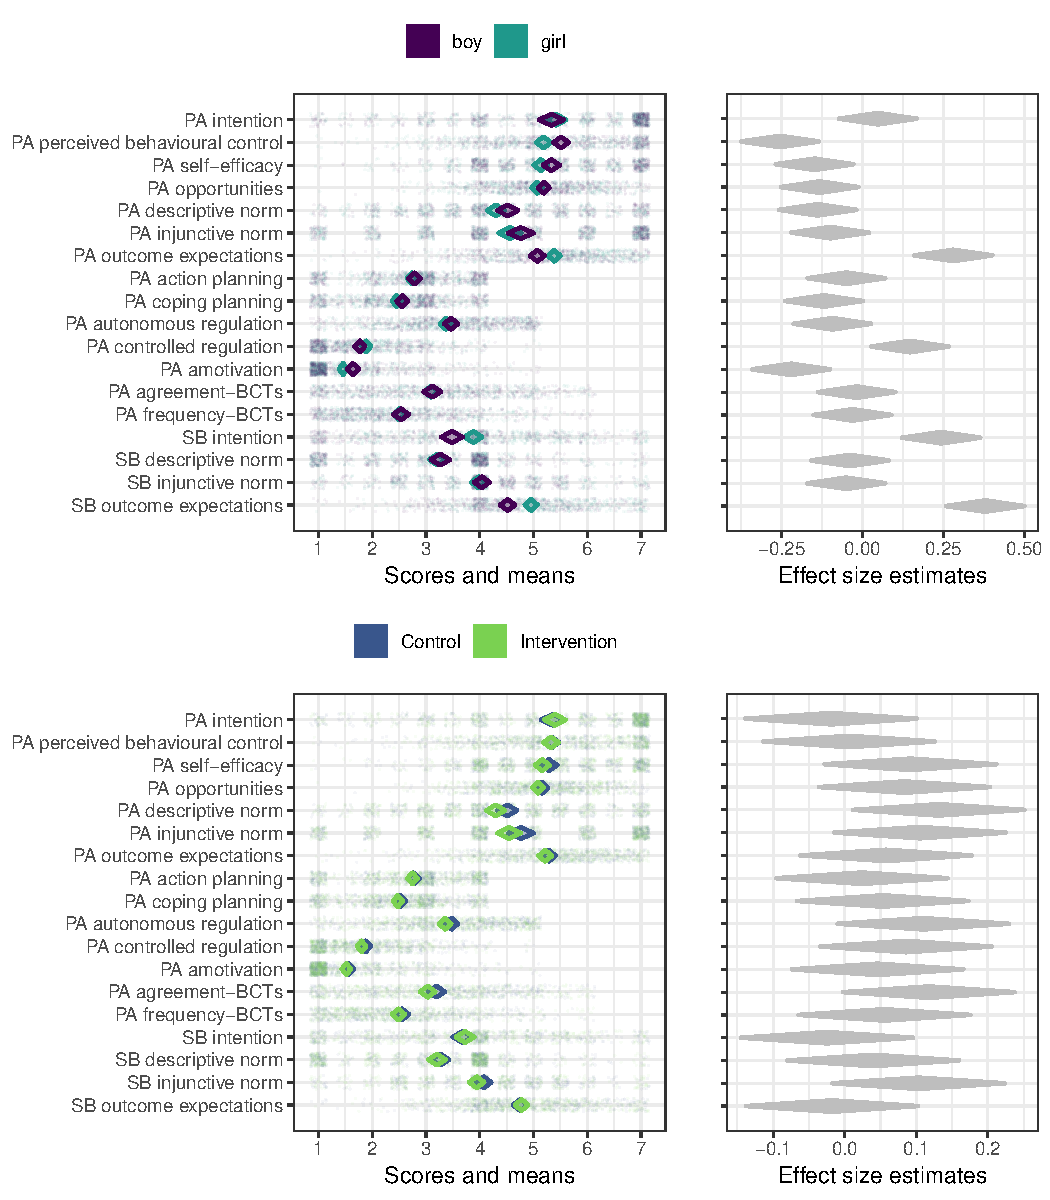
\includegraphics{_baseline-manuscript_files/figure-latex/determinant-diamondplot-manuscript-1.pdf}
\caption{\label{fig:determinant-diamondplot-manuscript}Diamond comparison plot drawn with R package \texttt{ufs} (code available at {[}add link to supplement's determinant-diamondplot{]}), showing means (middle of diamonds), 99\% confidence intervals (endpoints of diamonds) and individual answers (dots) separated by gender and arm. Rightmost plots show heuristic effect sizes for differences in means (transformed to Pearson's r). ICC is not accounted for in any plot. Nb. action and coping planning are evaluated on a scale from 1 to 4.}
\end{figure}

We can observe, for example, that SB descriptive norms are bimodal and thus the means are not representative of typical participants. In addition, several of the variables are skewed, which has implications on analytical choices as well as interpretations of the mean values.

\hypertarget{behaviour-change-technique-usage}{%
\subsubsection{Behaviour change technique usage}\label{behaviour-change-technique-usage}}

There were no clear differences between frequency-dependent BCT use between genders and arm (Figure \ref{fig:histogram-frequencyDependentBCTs}).

\begin{figure}
\centering
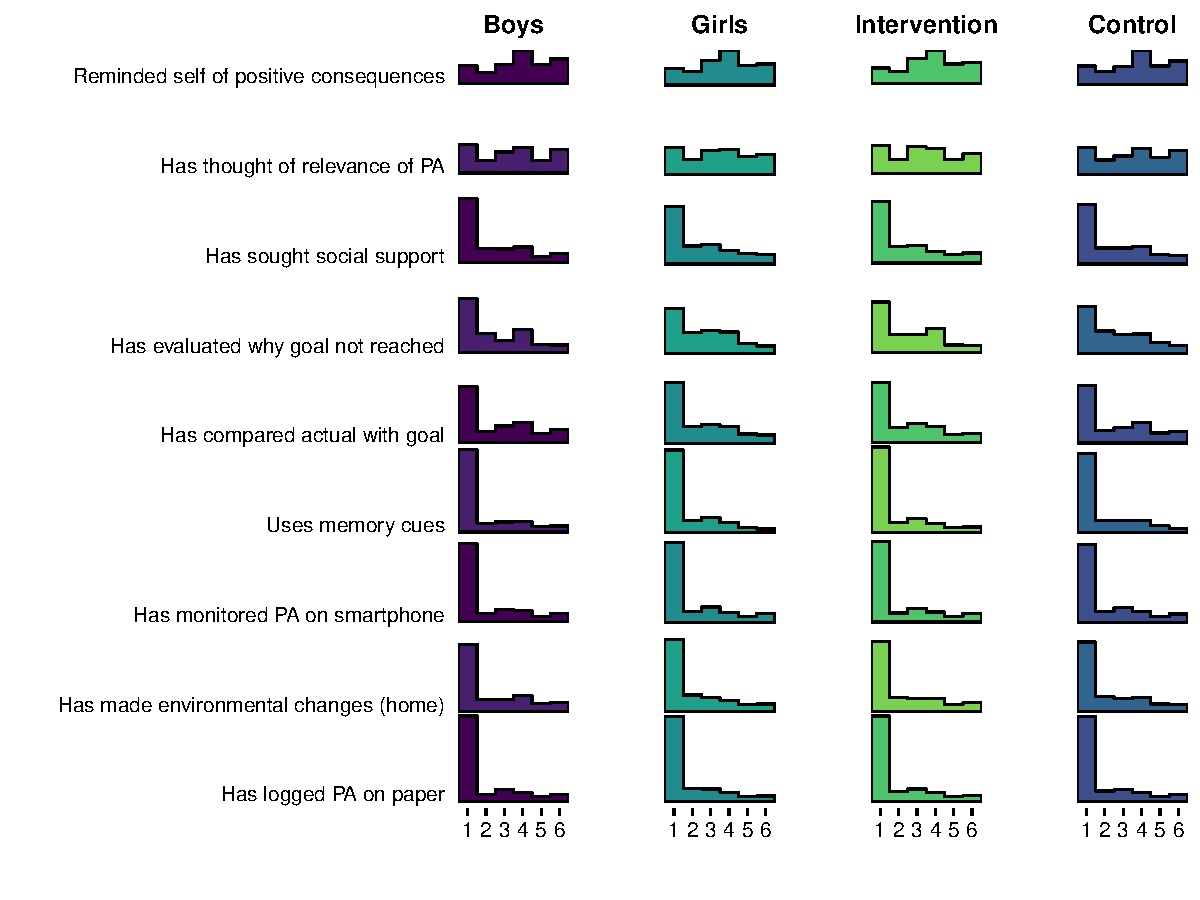
\includegraphics{_baseline-manuscript_files/figure-latex/histogram-frequencyDependentBCTs-1.pdf}
\caption{\label{fig:histogram-frequencyDependentBCTs}Histogram drawn with R package \texttt{ggridges} (code available at \url{https://git.io/fpOLj}), showing self-reported use of frequency-dependent BCTs (1 = Not once \ldots{} 6 = Daily).}
\end{figure}

Figure \ref{fig:histogram-frequencyDependentBCTs} tells that the most frequent response is 1, indicating non-use of that BCT. In fact, a large number of BCTs seem to indicate a composite distribution, where one population reports never using the BCT, and another is seems normally distributed around the middle of the scale.

The aforementioned forms can also be observed in the distributions of agreement-dependent BCTs, as presented in Figure \ref{fig:histogram-agreementDependentBCTs}.

\begin{figure}
\centering
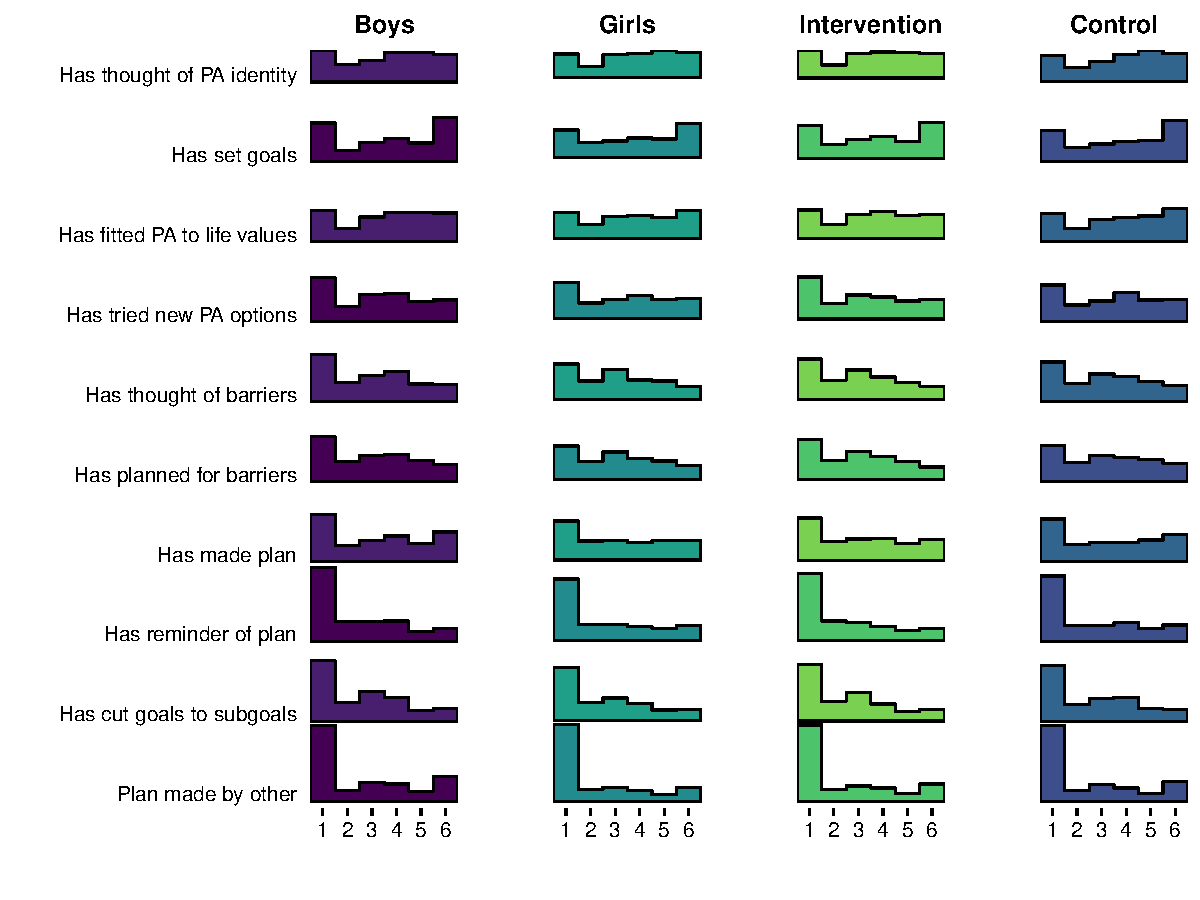
\includegraphics{_baseline-manuscript_files/figure-latex/histogram-agreementDependentBCTs-1.pdf}
\caption{\label{fig:histogram-agreementDependentBCTs}Histogram drawn with R package \texttt{ggridges} (code available at \url{https://git.io/fpOtq}), showing self-reported use of agreement-dependent BCTs (1 = Not at all true \ldots{} 6 = Completely true).}
\end{figure}

\hypertarget{demonstration-of-network-analysis}{%
\subsection{Demonstration of network analysis}\label{demonstration-of-network-analysis}}

Figure \ref{fig:network-plot} shows a LASSO regularised mixed graphical model of BCT use, motivation and the two MVPA measures. We can observe, that after taking into account all the other nodes in the network and regularising small connections to zero, autonomous motivation appears to serve as a link between many BCTs and MVPA. In fact, only having a plan made by someone else, and having tried out new ways to be physically active (during the past three weeks), are directly connected to either of the MVPA nodes. In addition, use of certain BCTs are coupled particularly closely: Strong links exist between goal setting and having an own PA plan, between identifying barriers and planning to overcome them (i.e.~problem solving), and between goal setting and an own PA plan. We can also see a triad, where reflecting positive consequences is connected to goal review, through having thought of personal reasons to do PA, as well as less strongly coupled social support and having made changes to home environment. These types of close connections can be indicative of underlying latent variables {[}60{]}.

\begin{figure}
\centering
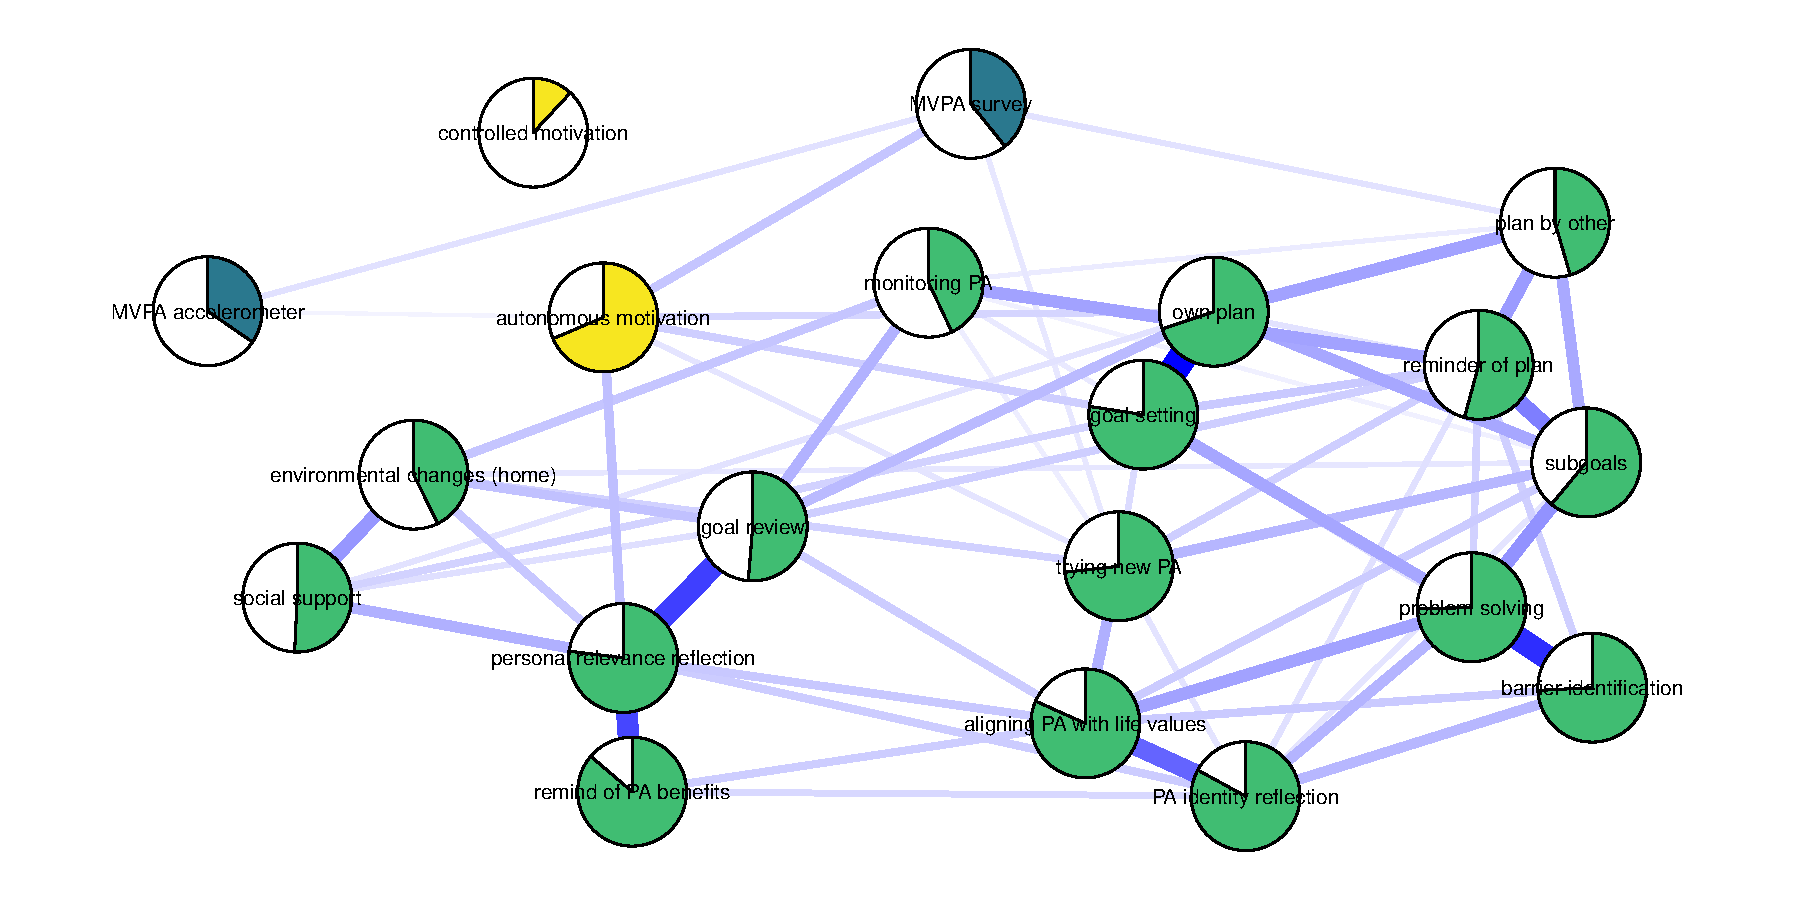
\includegraphics{_baseline-manuscript_files/figure-latex/network-plot-1.pdf}
\caption{\label{fig:network-plot}Mixed graphical model with LASSO regularisation and model selection by EBIC. Network models drawn with packages mgm and qgraph (code available at \url{https://git.io/fpOXV}). Blue lines indicate positive relationships. Plot shows the conditional dependence relationships between the variables of interest (edges which connect nodes), which can be interpreted akin to partial correlations. Pies depict means as proportion of theoretical maximum (in the case of accelerometer-measured MVPA, mean as proportion of highest observed value); BCT use and controlled motivation are dichotomised (see Methods).}
\end{figure}

\hypertarget{conclusions}{%
\section{Conclusions}\label{conclusions}}

This study investigated the baseline characteristics of the Let's Move It trial cohort, making use of modern tools to visualize key results and exhaustively report the analyses and findings and the analytical choices made. We found high levels of sedentary behaviour in the sample, with heterogeneity across educational tracks. MVPA, motivation and BCT use were modeled as a network, which highlighted the relevance of autonomous motivation in associations between PA and BCT use.

In contrast to earlier international and Finnish evidence collected in the general population (e.g.~{[}61{]}), girls performed more PA than boys in this sample. This is due to the practical nurse track being most active and mostly female; in other words, after accounting for track, no meaningful gender differences in accelerometer-measured MVPA could be seen. Further, boys reported doing more MVPA than girls, and the accelerometer-measurement implied they were also more sedentary and interrupted sitting less often. Intervention and control groups were similar in their accelerometer-measured MVPA. This observation supports the decision of pairing educational tracks in randomisation, such that all tracks were represented in both arms. The practical nurse track was simultaneously the largest, the most active and had the highest percentage of girls, which means that potential gender differences in eventual intervention results should be interpreted with caution.

To our knowledge, this is one of the first studies to measure the use of potential behaviour change techniques comprehensively already at the trial baseline. As can be expected, many people indeed do use BCTs even before the intervention takes place. The results reveal that in the past three weeks, many participants had not used self-regulation related BCTs such as planning, problem solving or goal setting, which on the other hand have been indicated to be useful techniques for PA self-management {[}62{]}. To our knowledge, this is also the first trial to measure the use of a range of BCTs also in the control arm participants which previous similar studies have failed to do.

Comprehensive, transparent reporting of results leads to a vast amount of information to be presented; visual exposition is thus vital. Visualising distributions makes it salient, how much variability there is among study participants, which informs us about the distributional assumptions, which underlie many of the statistical techniques we use. In addition, modern and traditional approaches to data visualisation allow us to go further than just comparing means, as well as provide opportunities to avoid drawing false conclusions (e.g.~in the case of Simpson's paradox) based on summary statistics.

The results of the network analysis highlight, how the effect of most naturally used BCTs on MVPA -- exceptions including having a plan made by someone else, and trying out new forms of PA -- are possibly mediated via autonomous motivation. This finding, if corroborated in longitudinal data, would support the theoretical framework of the intervention, which held autonomy support and behavioural experiments at the forefront. So far, network models have been largely used as a tool for exploring empirical relationships among variables, often with little existing theory {[}50,63{]}. One could understand this as the first generation of network papers in psychology, and there have been recent calls for a second generation that is confirmatory in nature, and based on existing theories of relationships among biological, psychological and social variables {[}47{]}.

The study also has limitations. It should be noted that while we consider 7-day accelerometry (more than 4 days of over 10 hours wear time) an approximation of a participant's true habitual PA and SB in their daily life, it is not an errorless measure of it, and does not capture all forms of activity. Additionally, the questionnaire to measure the BCTs requires future validation.

In the network model used, regularization techniques are applied to remove spurious relations and control for multiple testing (for an in-depth tutorial on such regularized network models, see {[}46{]}, and for a health psychology specific use case, see {[}58{]}). At the same time, these networks estimate relations that are akin to partial correlations to derive the conditional dependence structure among variables. Potential pitfalls of these models and their application have been discussed elsewhere in detail {[}47,64{]}. Most importantly, in social networks one can include all relevant nodes (e.g., all people in a classroom or company) in the network. This is not so in biopsychosocial networks, where the question of what items to include has turned out to be a challenging question. Relations among items are often interpreted as putative causal pathways (although many other interpretations exist, {[}46{]}), which means one should not include two variables that are simply two indicators of the same construct (e.g.~the items \enquote{I often feel sad} and \enquote{I often feel blue}). Another important challenge is that one should avoid statistically controlling for common effects, also known as colliders: If in the true model both A and B independently cause C, C is a collider. If one controls for C in the model, a negative relation between A and B will emerge where no relation exists in the true model. This applies to any regression models, and also in network models that are based on regressions, and it can be challenging to determine if a given variable is a collider. Rohrer {[}65{]} provides an approachable introduction to causal inference in observational data.

The type of supplement used for this manuscript allows for presenting a lot, but not all, information due to resource considerations. One of the reader groups not fully considered are researchers and educators, who wish to use these data to guide intervention design. We would like to point out that the results, like most of the research in the area, only provide a group-level snapshot of a wide variety of constantly unfolding dynamic processes. Few individual participants are described by the group-level summary statistics: In fact, using Daniels' {[}66{]} definition of an \enquote{approximately average individual} as falling in the middle 30\% of the range of values, only 1.20\% of participants can be considered \enquote{average} on all of the primary outcome measures (see supplementary website, section \url{https://git.io/fpOy1}). Intervention designers looking at this cohort to choose to-be-targeted determinants for their study, may want to consider applying clustering techniques on the data once it becomes publicly available. Still, and especially when processes are considered, group-level data does not inform the individual-level mechanisms of action in the case of non-ergodic systems, and hence the agreement between features of these two levels should be investigated {[}67{]}.

In conclusion, this analysis of baseline data from the Let's Move It intervention trial indicates that randomization did not result in highly disproportionate groups, i.e.~the differences between arms were minimal -- although, in the case of complex systems, even small differences may proliferate and lead to group imbalances {[}68{]}. It also has highlighted that the vocational school students differ in many regards by their chosen educational track. Finally, graphical methods of presenting descriptive data are an important addition to traditional tables displaying means and standard deviations, and transparent sharing of analyses and analytical choices is imperative for increasing confidence in research findings.

\hypertarget{list-of-abbreviations}{%
\subsubsection{List of abbreviations}\label{list-of-abbreviations}}

MVPA moderate-to-vigorous physical activity\\
SB sedentary behavior\\
Nur = Practical nurse\\
HRC = Hotel, restaurant and catering studies\\
BA = Business and administration\\
IT = Business information technology

\hypertarget{declarations}{%
\subsection{Declarations}\label{declarations}}

\hypertarget{ethics-approval-and-consent-to-participate}{%
\subsubsection{Ethics approval and consent to participate}\label{ethics-approval-and-consent-to-participate}}

The research proposal was reviewed by the Ethics Committee for Gynaecology and Obstetrics, Pediatrics and Psychiatry of the Hospital District of Helsinki and Uusimaa (decision number 367/13/03/03/2014).

\hypertarget{availability-of-data-and-materials}{%
\subsubsection{Availability of data and materials}\label{availability-of-data-and-materials}}

The analysis data will be available at {[}OSF storage{]} on 1st July 2019. All analyses and code are available at \url{https://git.io/fNHuf} (permalink at {[}REF{]}, repository at {[}REF{]}).

\hypertarget{competing-interests}{%
\subsubsection{Competing interests}\label{competing-interests}}

The authors declare that they have no competing interests.

\hypertarget{authors-contributions}{%
\subsubsection{Authors' contributions}\label{authors-contributions}}

MH wrote the analysis code, including the full online supplement, formulated the initial draft of the manuscript and revised it in collaboration with all co-authors. TV was responsible for planning and analysing the PA and SB measured from data collected with accelerometer. RS and EIF provided expertise regarding the statistical analyses. KB, AH, AU, VA, TV, RS and NH contributed to planning of the trial design and data collection including the measures used. NH conceived of the study and acted as principal investigator of the research project. All authors read and approved the final manuscript.

\hypertarget{funding}{%
\subsubsection{Funding}\label{funding}}

MH was supported by Academy of Finland (grant number 295765) and Ministry for Education and Culture, Sports Science projects (grant number OKM/81/626/2014). NH was supported by an Academy of Finland Research Fellowship (grant number 285283). The data were collected in a project funded by Ministry for Education and Culture, Sports Science projects (grant number OKM/81/626/2014).

\hypertarget{acknowledgements}{%
\subsubsection{Acknowledgements}\label{acknowledgements}}

We would like to thank participating schools, their staff and students, as well as the numerous people who have helped in study design and data collection.

\newpage

\hypertarget{references}{%
\section{References}\label{references}}

\begingroup
\setlength{\parindent}{-0.5in}
\setlength{\leftskip}{0.5in}

\hypertarget{refs}{}
\leavevmode\hypertarget{ref-elgarSocioeconomicInequalitiesAdolescent2015}{}%
1. Elgar FJ, Pförtner T-K, Moor I, De Clercq B, Stevens GWJM, Currie C. Socioeconomic inequalities in adolescent health 2002--2010: A time-series analysis of 34 countries participating in the Health Behaviour in School-aged Children study. The Lancet {[}Internet{]}. 2015 {[}cited 2016 Feb 24{]};385:2088--95. Available from: \url{http://linkinghub.elsevier.com/retrieve/pii/S0140673614614604}

\leavevmode\hypertarget{ref-dielemanTrendsFutureHealth2018}{}%
2. Dieleman JL, Sadat N, Chang AY, Fullman N, Abbafati C, Acharya P, et al. Trends in future health financing and coverage: Future health spending and universal health coverage in 188 countries, 2016--40. The Lancet. 2018;391:1783--98.

\leavevmode\hypertarget{ref-husuObjectivelyMeasuredSedentary2016}{}%
3. Husu P, Vähä-Ypyä H, Vasankari T. Objectively measured sedentary behavior and physical activity of Finnish 7-to 14-year-old children--associations with perceived health status: A cross-sectional study. BMC public health. 2016;16:338.

\leavevmode\hypertarget{ref-makelaPhysicalActivityScreen2016}{}%
4. Mäkelä K, Kokko S, Kannas L, Villberg J, Vasankari T, Heinonen JO, et al. Physical Activity, Screen Time and Sleep among Youth Participating and Non-Participating in Organized Sports: The Finnish Health Promoting Sports Club (FHPSC) Study. Advances in Physical Education. 2016;6.

\leavevmode\hypertarget{ref-vansluijsPhysicalActivityDietary2008}{}%
5. van Sluijs EM, Skidmore PM, Mwanza K, Jones AP, Callaghan AM, Ekelund U, et al. Physical activity and dietary behaviour in a population-based sample of British 10-year old children: The SPEEDY study (Sport, Physical activity and Eating behaviour: Environmental Determinants in Young people). BMC public health. 2008;8:388.

\leavevmode\hypertarget{ref-hankonenWhatExplainsSocioeconomic2017}{}%
6. Hankonen N, Heino MT, Kujala E, Hynynen S-T, Absetz P, Ara\a'ujo-Soares V, et al. What explains the socioeconomic status gap in activity? Educational differences in determinants of physical activity and screentime. BMC public health {[}Internet{]}. 2017 {[}cited 2017 May 27{]};17:144. Available from: \url{https://bmcpublichealth.biomedcentral.com/articles/10.1186/s12889-016-3880-5}

\leavevmode\hypertarget{ref-hynynenSystematicReviewSchoolbased2016}{}%
7. Hynynen S-T, van Stralen MM, Sniehotta FF, Ara\a'ujo-Soares V, Hardeman W, Chinapaw MJM, et al. A systematic review of school-based interventions targeting physical activity and sedentary behaviour among older adolescents. Int Rev Sport Exerc Psychol. 2016;9:22--44.

\leavevmode\hypertarget{ref-mooreProcessEvaluationComplex2015}{}%
8. Moore GF, Audrey S, Barker M, Bond L, Bonell C, Hardeman W, et al. Process evaluation of complex interventions: Medical Research Council guidance. BMJ. 2015;350:h1258.

\leavevmode\hypertarget{ref-rogersUsingProgrammeTheory2008a}{}%
9. Rogers PJ. Using Programme Theory to Evaluate Complicated and Complex Aspects of Interventions. Evaluation. 2008;14:29--48.

\leavevmode\hypertarget{ref-hankonenRandomisedControlledFeasibility2017}{}%
10. Hankonen N, Heino MTJ, Hynynen S-T, Laine H, Ara\a'ujo-Soares V, Sniehotta FF, et al. Randomised controlled feasibility study of a school-based multi-level intervention to increase physical activity and decrease sedentary behaviour among vocational school students. International Journal of Behavioral Nutrition and Physical Activity. 2017;14.

\leavevmode\hypertarget{ref-koykkaCombiningReasonedAction2018}{}%
11. Köykkä K, Absetz P, AraÃ\textordmasculinejo-Soares V, Knittle K, Sniehotta FF, Hankonen N. Combining the reasoned action approach and habit formation to reduce sitting time in classrooms: Outcome and process evaluation of the Let's Move It teacher intervention. Journal of Experimental Social Psychology. 2018;

\leavevmode\hypertarget{ref-clevelandVisualizingData1993}{}%
12. Cleveland WS. Visualizing data. Hobart Press; 1993.

\leavevmode\hypertarget{ref-tukeyExploratoryDataAnalysis1977}{}%
13. Tukey JW. Exploratory data analysis. Reading, Mass. 1977.

\leavevmode\hypertarget{ref-saxonBarCharts2015}{}%
14. Saxon E. Beyond bar charts. BMC Biology. 2015;13:60.

\leavevmode\hypertarget{ref-weissgerberBarLineGraphs2015}{}%
15. Weissgerber TL, Milic NM, Winham SJ, Garovic VD. Beyond Bar and Line Graphs: Time for a New Data Presentation Paradigm. PLOS Biology. 2015;13:e1002128.

\leavevmode\hypertarget{ref-weissgerberStaticInteractiveTransforming2016}{}%
16. Weissgerber TL, Garovic VD, Savic M, Winham SJ, Milic NM. From Static to Interactive: Transforming Data Visualization to Improve Transparency. PLOS Biology. 2016;14:e1002484.

\leavevmode\hypertarget{ref-tayGraphicalDescriptivesWay2016}{}%
17. Tay L, Parrigon S, Huang Q, LeBreton JM. Graphical Descriptives A Way to Improve Data Transparency and Methodological Rigor in Psychology. Perspectives on Psychological Science. 2016;11:692--701.

\leavevmode\hypertarget{ref-chalmersAvoidableWasteProduction2009}{}%
18. Chalmers I, Glasziou P. Avoidable waste in the production and reporting of research evidence. Lancet. 2009;374:86--9.

\leavevmode\hypertarget{ref-boardofgovernorsofthefederalreservesystemEconomicsResearchReplicable2015}{}%
19. Board of Governors of the Federal Reserve System, Chang AC, Li P. Is Economics Research Replicable? Sixty Published Papers from Thirteen Journals Say "Usually Not". Finance and Economics Discussion Series. 2015;2015:1--26.

\leavevmode\hypertarget{ref-bondSadTruthHappiness2018}{}%
20. Bond TN, Lang K. The Sad Truth About Happiness Scales: Empirical Results. National Bureau of Economic Research; 2018 Jul. Report No.: 24853.

\leavevmode\hypertarget{ref-gigerenzerStatisticalRitualsReplication2018}{}%
21. Gigerenzer G. Statistical Rituals: The Replication Delusion and How We Got There. Advances in Methods and Practices in Psychological Science. 2018;2515245918771329.

\leavevmode\hypertarget{ref-kepesHowTrustworthyScientific2013}{}%
22. Kepes S, McDaniel MA. How Trustworthy Is the Scientific Literature in Industrial and Organizational Psychology? Industrial and Organizational Psychology. 2013;6:252--68.

\leavevmode\hypertarget{ref-nosekPreregistrationRevolution2018}{}%
23. Nosek BA, Ebersole CR, DeHaven AC, Mellor DT. The preregistration revolution. Proceedings of the National Academy of Sciences. 2018;201708274.

\leavevmode\hypertarget{ref-nosekScientificUtopiaII2012}{}%
24. Nosek BA, Spies JR, Motyl M. Scientific Utopia II. Restructuring Incentives and Practices to Promote Truth Over Publishability. Perspectives on Psychological Science. 2012;7:615--31.

\leavevmode\hypertarget{ref-simmonsFalsePositivePsychologyUndisclosed2011}{}%
25. Simmons JP, Nelson LD, Simonsohn U. False-Positive Psychology Undisclosed Flexibility in Data Collection and Analysis Allows Presenting Anything as Significant. Psychological Science. 2011;22:1359--66.

\leavevmode\hypertarget{ref-smaldinoNaturalSelectionBad2016}{}%
26. Smaldino PE, McElreath R. The natural selection of bad science. Open Science. 2016;3:160384.

\leavevmode\hypertarget{ref-stoddenEmpiricalAnalysisJournal2018}{}%
27. Stodden V, Seiler J, Ma Z. An empirical analysis of journal policy effectiveness for computational reproducibility. Proceedings of the National Academy of Sciences. 2018;115:2584--9.

\leavevmode\hypertarget{ref-nosekReproducibilityCancerBiology2017}{}%
28. Nosek BA, Errington TM. Reproducibility in cancer biology: Making sense of replications. Elife. 2017;6:e23383.

\leavevmode\hypertarget{ref-expertadvisorygroupondataaccessEAGDAReportGovernance2015}{}%
29. Expert Advisory Group on Data Access. EAGDA Report: Governance of Data Access. the Wellcome Trust; 2015.

\leavevmode\hypertarget{ref-vanpaemelAreWeWasting2015}{}%
30. Vanpaemel W, Vermorgen M, Deriemaecker L, Storms G. Are We Wasting a Good Crisis? The Availability of Psychological Research Data after the Storm. Collabra: Psychology. 2015;1.

\leavevmode\hypertarget{ref-hallgrenPathDiagramsEnhancing2018}{}%
31. Hallgren KA, McCabe CJ, King KM, Atkins DC. Beyond path diagrams: Enhancing applied structural equation modeling research through data visualization. Addictive Behaviors. 2018;

\leavevmode\hypertarget{ref-rcoreteamLanguageEnvironmentStatistical2017}{}%
32. R Core Team. R: A Language and Environment for Statistical Computing. Vienna, Austria: R Foundation for Statistical Computing; 2017.

\leavevmode\hypertarget{ref-hankonenLetMoveIt2016}{}%
33. Hankonen N, Heino MTJ, Araujo-Soares V, Sniehotta FF, Sund R, Vasankari T, et al. ``Let's Move It'' a school-based multilevel intervention to increase physical activity and reduce sedentary behaviour among older adolescents in vocational secondary schools: A study protocol for a cluster-randomised trial. BMC Public Health. 2016;16:451--66.

\leavevmode\hypertarget{ref-fagtNordicMonitoringDiet2012}{}%
34. Fagt S, Andersen LF, Anderssen SA, Becker W, Borodulin K, Fogelholm M, et al. Nordic Monitoring of diet, physical activity and overweight : Validation of indicators. Nordic Council of Ministers; 2012.

\leavevmode\hypertarget{ref-vaha-ypyaUniversalAccurateIntensitybased2015}{}%
35. Vähä-Ypyä H, Vasankari T, Husu P, Suni J, Sievänen H. A universal, accurate intensity-based classification of different physical activities using raw data of accelerometer. Clinical physiology and functional imaging. 2015;35:64--70.

\leavevmode\hypertarget{ref-vaha-ypyaValidationCutpointsEvaluating2015}{}%
36. Vähä-Ypyä H, Vasankari T, Husu P, Mänttäri A, Vuorimaa T, Suni J, et al. Validation of cut-points for evaluating the intensity of physical activity with accelerometry-based mean amplitude deviation (MAD). PLoS One. 2015;10:e0134813.

\leavevmode\hypertarget{ref-tremblaySedentaryBehaviorResearch2017}{}%
37. Tremblay MS, Aubert S, Barnes JD, Saunders TJ, Carson V, Latimer-Cheung AE, et al. Sedentary Behavior Research Network (SBRN) process and outcome. International Journal of Behavioral Nutrition and Physical Activity. 2017;14:75.

\leavevmode\hypertarget{ref-vaha-ypyaReliableRecognitionLying2018}{}%
38. Vähä-Ypyä H, Husu P, Suni J, Vasankari T, Sievänen H. Reliable recognition of lying, sitting, and standing with a hip-worn accelerometer. Scandinavian Journal of Medicine \& Science in Sports. 2018;28:1092--102.

\leavevmode\hypertarget{ref-rstudioteamRStudioIntegratedDevelopment2016}{}%
39. RStudio Team. RStudio: Integrated Development Environment for R. Boston, MA: RStudio, Inc. 2016.

\leavevmode\hypertarget{ref-R-base}{}%
40. R Core Team. R: A language and environment for statistical computing {[}Internet{]}. Vienna, Austria: R Foundation for Statistical Computing; 2018. Available from: \url{https://www.R-project.org/}

\leavevmode\hypertarget{ref-gardnerConfidenceIntervalsRather1986}{}%
41. Gardner MJ, Altman DG. Confidence intervals rather than P values: Estimation rather than hypothesis testing. BMJ. 1986;292:746--50.

\leavevmode\hypertarget{ref-sterneSiftingEvidenceWhat2001}{}%
42. Sterne JAC. Sifting the evidence---what's wrong with significance tests? Another comment on the role of statistical methods. BMJ. 2001;322:226--31.

\leavevmode\hypertarget{ref-wassersteinASAStatementPValues2016}{}%
43. Wasserstein RL, Lazar NA. The ASA's Statement on p-Values: Context, Process, and Purpose. The American Statistician. 2016;70:129--33.

\leavevmode\hypertarget{ref-haslbeckStructureEstimationMixed2015}{}%
44. Haslbeck J, Waldorp LJ. Structure estimation for mixed graphical models in high-dimensional data. arXiv preprint arXiv:151005677. 2015;

\leavevmode\hypertarget{ref-tibshiraniRegressionShrinkageSelection1996}{}%
45. Tibshirani R. Regression shrinkage and selection via the lasso: A retrospective. Journal of the Royal Statistical Society: Series B (Statistical Methodology). 1996;73:273--82.

\leavevmode\hypertarget{ref-epskampTutorialRegularizedPartial2018}{}%
46. Epskamp S, Fried EI. A Tutorial on Regularized Partial Correlation Networks. Psychological Methods {[}Internet{]}. 2018; Available from: \url{http://arxiv.org/abs/1607.01367}

\leavevmode\hypertarget{ref-friedMovingForwardChallenges2017}{}%
47. Fried EI, Cramer AO. Moving forward: Challenges and directions for psychopathological network theory and methodology. Perspectives on Psychological Science. 2017;12:999--1020.

\leavevmode\hypertarget{ref-dalegeFormalizedAccountAttitudes2016}{}%
48. Dalege J, Borsboom D, van Harreveld F, van den Berg H, Conner M, van der Maas HLJ. Toward a formalized account of attitudes: The Causal Attitude Network (CAN) model. Psychological Review. 2016;123:2--22.

\leavevmode\hypertarget{ref-dalegeNetworkStructureExplains2017}{}%
49. Dalege J, Borsboom D, Harreveld F, Waldorp LJ, Maas HL. Network structure explains the impact of attitudes on voting decisions. Scientific reports. 2017;7:4909.

\leavevmode\hypertarget{ref-mottusWhyTraitsCome2017}{}%
50. Mõttus R, Allerhand M. Why do traits come together? The underlying trait and network approaches. SAGE handbook of personality and individual differences. 2017;1:1--22.

\leavevmode\hypertarget{ref-vandermaasNetworkModelsCognitive2017}{}%
51. Van Der Maas H, Kan K-J, Marsman M, Stevenson CE. Network Models for Cognitive Development and Intelligence. 2017.

\leavevmode\hypertarget{ref-friedMentalDisordersNetworks2017}{}%
52. Fried EI, van Borkulo CD, Cramer AO, Boschloo L, Schoevers RA, Borsboom D. Mental disorders as networks of problems: A review of recent insights. Social Psychiatry and Psychiatric Epidemiology. 2017;52:1--10.

\leavevmode\hypertarget{ref-brigantiNetworkAnalysisEmpathy2018}{}%
53. Briganti G, Kempenaers C, Braun S, Fried EI, Linkowski P. Network analysis of empathy items from the interpersonal reactivity index in 1973 young adults. Psychiatry Research. 2018;265:87--92.

\leavevmode\hypertarget{ref-dalegeNetworkAnalysisAttitudes2017}{}%
54. Dalege J, Borsboom D, van Harreveld F, van der Maas HL. Network analysis on attitudes: A brief tutorial. Social psychological and personality science. 2017;8:528--37.

\leavevmode\hypertarget{ref-epskampEstimatingPsychologicalNetworks2016}{}%
55. Epskamp S, Borsboom D, Fried EI. Estimating Psychological Networks and their Stability: A Tutorial Paper. arXiv preprint arXiv:160408462. 2016;

\leavevmode\hypertarget{ref-costantiniStateARtPersonality2015}{}%
56. Costantini G, Epskamp S, Borsboom D, Perugini M, Mõttus R, Waldorp LJ, et al. State of the aRt personality research: A tutorial on network analysis of personality data in R. Journal of Research in Personality. 2015;54:13--29.

\leavevmode\hypertarget{ref-costantiniStabilityVariabilityPersonality2017}{}%
57. Costantini G, Richetin J, Preti E, Casini E, Epskamp S, Perugini M. Stability and variability of personality networks. A tutorial on recent developments in network psychometrics. Personality and Individual Differences. 2017;

\leavevmode\hypertarget{ref-heveyNetworkAnalysisBrief2018}{}%
58. Hevey D. Network analysis: A brief overview and tutorial. Health Psychology and Behavioral Medicine. 2018;6:301--28.

\leavevmode\hypertarget{ref-kievitSimpsonParadoxPsychological2013}{}%
59. Kievit RA, Frankenhuis WE, Waldorp LJ, Borsboom D. Simpson's paradox in psychological science: A practical guide. Frontiers in Psychology. 2013;4.

\leavevmode\hypertarget{ref-molenaarLatentVariableModels2010}{}%
60. Molenaar PCM. Latent variable models are network models. Behavioral and Brain Sciences. 2010;33:166--6.

\leavevmode\hypertarget{ref-husuObjectivelyMeasuredSedentary2016a}{}%
61. Husu P, Suni J, VÃ\textcurrencyhÃ\textcurrency-YpyÃ\textcurrency H, Sievänen H, Tokola K, Valkeinen H, et al. Objectively measured sedentary behavior and physical activity in a sample of Finnish adults: A cross-sectional study. BMC Public Health. 2016;16.

\leavevmode\hypertarget{ref-michieEffectiveTechniquesHealthy2009}{}%
62. Michie S, Abraham C, Whittington C, McAteer J, Gupta S. Effective techniques in healthy eating and physical activity interventions: A meta-regression. Health Psychology. 2009;28:690--701.

\leavevmode\hypertarget{ref-friedMentalDisordersNetworks2017a}{}%
63. Fried EI, van Borkulo CD, Cramer AOJ, Boschloo L, Schoevers RA, Borsboom D. Mental disorders as networks of problems: A review of recent insights. Social Psychiatry and Psychiatric Epidemiology. 2017;52:1--10.

\leavevmode\hypertarget{ref-guloksuzApplicationNetworkMethods2017}{}%
64. Guloksuz S, Pries LK, Van Os J. Application of network methods for understanding mental disorders: Pitfalls and promise. Psychological medicine. 2017;47:2743--52.

\leavevmode\hypertarget{ref-rohrerThinkingClearlyCorrelations2018}{}%
65. Rohrer JM. Thinking Clearly About Correlations and Causation: Graphical Causal Models for Observational Data. Advances in Methods and Practices in Psychological Science. 2018;1:27--42.

\leavevmode\hypertarget{ref-danielsAverageMan1952}{}%
66. Daniels GS. The" Average Man"? AIR FORCE AEROSPACE MEDICAL RESEARCH LAB WRIGHT-PATTERSON AFB OH; 1952.

\leavevmode\hypertarget{ref-fisherLackGrouptoindividualGeneralizability2018}{}%
67. Fisher AJ, Medaglia JD, Jeronimus BF. Lack of group-to-individual generalizability is a threat to human subjects research. Proceedings of the National Academy of Sciences. 2018;201711978.

\leavevmode\hypertarget{ref-ricklesCausalityComplexInterventions2009}{}%
68. Rickles D. Causality in complex interventions. Medicine, Health Care, and Philosophy. 2009;12:77--90.

\endgroup


\end{document}
